\chapter{Full Regime Catalogue}
\label{app:full_regime_catalogue}

This appendix collects all systematic experiment configurations,
together with their dynamics parameters and summary
$R^2$ for MVAR and LSTM\@.  Of the 54 YAML configurations in
\texttt{configs/systematic/}, six were excluded before running
(three near-duplicate base regimes---NDYN03, NDYN11,
NDYN12---and their VS counterparts), leaving 48 candidates.
The table also includes tier-1 sensitivity variants and
preprocessing ablations where available.  The nine primary benchmark
regimes from Chapters~\ref{ch:rom_results} and~\ref{ch:wsindy_results}
are shown in bold.

% -----------------------------------------------------------------------
\section{Dynamics parameters and ROM accuracy}
\label{sec:regime_catalogue_table}
% -----------------------------------------------------------------------

Table~\ref{tab:full_regime_catalogue} lists every systematic regime.
The CS and VS variants share the same force parameters but differ in speed
coupling.  Tables~\ref{tab:ndyn_regimes_full} and~\ref{tab:do_regimes_full}
give the governing parameters.

% Two-column tabular layout; wrapped in a table float
\begin{table}[htbp]
\centering
\caption{Mean test $R^2$ for MVAR and LSTM across all systematic experiments.
Bold = nine main-text regimes; ---$^\dagger$ = LSTM diverged ($R^2<{-}2$);
--- = not yet available.}
\label{tab:full_regime_catalogue}
\scriptsize\setlength{\tabcolsep}{3pt}
\noindent
\begin{minipage}[t]{0.49\textwidth}
\begin{tabular}{@{}lrr@{}}
\hline
Regime & MVAR $R^2$ & LSTM $R^2$ \\
\hline
DO\_CS01\_swarm\_C01\_l05 & 0.949 & 0.920 \\
DO\_CS01\_swarm\_C01\_l05\_VS & 0.594 & -0.702 \\
DO\_CS02\_swarm\_C05\_l3 & 0.094 & 0.109 \\
DO\_CS03\_swarm\_C09\_l3 & 0.228 & 0.130 \\
DO\_DM01\_dmill\_C09\_l05 & 0.992 & -0.000 \\
DO\_DM01\_dmill\_C09\_l05\_VS & 0.807 & -0.909 \\
DO\_DR01\_dring\_C01\_l01 & 0.953 & 0.612 \\
DO\_DR01\_dring\_C01\_l01\_VS & 0.538 & -0.695 \\
DO\_DR02\_dring\_C09\_l09 & 0.984 & 0.984 \\
DO\_DR02\_dring\_C09\_l09\_VS & 0.574 & -0.838 \\
DO\_EC01\_esccol\_C2\_l3 & --- & --- \\
DO\_EC02\_esccol\_C3\_l05 & 0.423 & -0.490 \\
DO\_EC02\_esccol\_C3\_l05\_VS & 0.133 & ---$^\dagger$ \\
DO\_ES01\_escsym\_C3\_l09 & 0.629 & 0.026 \\
DO\_ES01\_escsym\_C3\_l09\_VS & -0.004 & -0.409 \\
DO\_EU01\_escuns\_C2\_l2 & 0.446 & 0.437 \\
DO\_EU01\_escuns\_C2\_l2\_VS & 0.102 & 0.015 \\
DO\_EU02\_escuns\_C3\_l3 & --- & --- \\
DO\_SM01\_mill\_C05\_l01 & 0.992 & -0.206 \\
DO\_SM01\_mill\_C05\_l01\_VS & 0.483 & -0.840 \\
DO\_SM02\_mill\_C3\_l01 & 0.939 & 0.936 \\
DO\_SM02\_mill\_C3\_l01\_VS & 0.252 & -1.141 \\
DO\_SM03\_mill\_C2\_l05 & 0.990 & 0.178 \\
DO\_SM03\_mill\_C2\_l05\_VS & 0.557 & -1.120 \\
NDYN01\_crawl & 0.980 & -0.133 \\
NDYN01\_crawl\_VS & 0.676 & 0.187 \\
NDYN02\_flock & 0.956 & 0.415 \\
NDYN02\_flock\_VS & 0.271 & -0.465 \\
\hline
\end{tabular}
\end{minipage}\hfill
\begin{minipage}[t]{0.49\textwidth}
\begin{tabular}{@{}lrr@{}}
\hline
Regime & MVAR $R^2$ & LSTM $R^2$ \\
\hline
\textbf{NDYN04\_gas\_VS} & \textbf{0.558} & \textbf{0.110} \\
NDYN04\_gas\_VS\_tier1\_bic & 0.491 & -0.702 \\
NDYN04\_gas\_VS\_tier1\_w5 & 0.410 & 0.110 \\
NDYN04\_gas\_preproc\_sqrt\_none & --- & 0.990 \\
NDYN04\_gas\_preproc\_sqrt\_scale & --- & 0.950 \\
\textbf{NDYN04\_gas} & \textbf{0.996} & \textbf{0.996} \\
NDYN04\_gas\_tier1\_bic & 0.989 & 0.676 \\
NDYN04\_gas\_tier1\_w5 & 0.990 & 0.657 \\
\textbf{NDYN05\_blackhole\_VS} & \textbf{0.704} & \textbf{-0.214} \\
NDYN05\_blackhole\_VS\_tier1\_bic & -1.269 & -1.484 \\
NDYN05\_blackhole\_VS\_tier1\_w5 & -1.040 & ---$^\dagger$ \\
\textbf{NDYN05\_blackhole} & \textbf{0.994} & \textbf{0.992} \\
NDYN05\_blackhole\_tier1\_bic & 0.992 & 0.987 \\
NDYN05\_blackhole\_tier1\_w5 & 0.993 & 0.791 \\
\textbf{NDYN06\_supernova\_VS} & \textbf{0.244} & \textbf{0.163} \\
\textbf{NDYN06\_supernova} & \textbf{0.683} & \textbf{0.508} \\
NDYN06\_supernova\_tier1\_bic & 0.528 & 0.291 \\
NDYN06\_supernova\_tier1\_w5 & 0.683 & -1.289 \\
\textbf{NDYN07\_crystal\_VS} & \textbf{0.292} & \textbf{-0.779} \\
\textbf{NDYN07\_crystal} & \textbf{0.996} & \textbf{0.585} \\
\textbf{NDYN08\_pure\_vicsek} & \textbf{0.654} & \textbf{0.229} \\
NDYN09\_longrange & --- & --- \\
NDYN10\_shortrange & --- & --- \\
NDYN10\_shortrange\_VS & 0.402 & ---$^\dagger$ \\
NDYN13\_chaos & 0.974 & 0.851 \\
NDYN13\_chaos\_VS & 0.290 & -0.592 \\
NDYN14\_varspeed & 0.287 & ---$^\dagger$ \\
\hline
\end{tabular}
\end{minipage}

\end{table}

Tables~\ref{tab:ndyn_regimes_full} and~\ref{tab:do_regimes_full} give the
full parameter sets; each base config also has a \texttt{\_VS} variant
unless noted.

\begin{table}[ht]
\centering
\caption{NDYN regimes (full catalogue).  Bold = main-text benchmarks;
  $\dagger$ = removed near-duplicates.}
\label{tab:ndyn_regimes_full}
\scriptsize\renewcommand{\arraystretch}{0.85}
\begin{tabular}{llrrrrrrl}
\hline
Label & Nickname & $v_0$ & $\eta$ & $C_a$ & $C_r$ & $\ell_a$ & $\ell_r$ & Notes \\
\hline
NDYN01 & crawl       & 0.5 & 0.03 & 0.8  & 0.3  & 1.5 & 0.5 & easy POD baseline \\
NDYN02 & flock       & 3.0 & 0.1  & 2.0  & 0.5  & 1.5 & 0.5 & coherent cluster \\
NDYN03$^\dagger$ & sprint      & 10.0& 0.1  & 2.0  & 0.5  & 1.5 & 0.5 & \textit{removed (dup.\ NDYN02)} \\
\textbf{NDYN04} & \textbf{gas} & \textbf{3.0} & \textbf{1.5} & \textbf{0.5} & \textbf{0.2} & \textbf{1.5} & \textbf{0.5} & \textbf{disordered gas} \\
\textbf{NDYN05} & \textbf{blackhole} & \textbf{4.0} & \textbf{0.15} & \textbf{20.0} & \textbf{0.05} & \textbf{1.5} & \textbf{0.3} & \textbf{near-singular spike} \\
\textbf{NDYN06} & \textbf{supernova} & \textbf{3.0} & \textbf{0.15} & \textbf{0.05} & \textbf{15.0} & \textbf{1.5} & \textbf{0.5} & \textbf{explosive repulsion} \\
\textbf{NDYN07} & \textbf{crystal}     & \textbf{2.0} & \textbf{0.1}  & \textbf{3.0}  & \textbf{3.0}  & \textbf{2.0} & \textbf{0.5} & \textbf{balanced equilibrium} \\
\textbf{NDYN08} & \textbf{pure Vicsek} & \textbf{3.0} & \textbf{0.3} & \textbf{---} & \textbf{---} & \textbf{---} & \textbf{---} & \textbf{forces off} \\
NDYN09 & longrange   & 2.0 & 0.2  & 1.5  & 0.6  & 6.0 & 3.0 & global collective modes \\
NDYN10 & shortrange  & 3.0 & 0.15 & 4.0  & 2.0  & 0.3 & 0.1 & fragmented clusters \\
NDYN11$^\dagger$ & noisy collapse & 3.0 & 0.8 & 12.0 & 0.1 & 1.5 & 0.5 & \textit{removed (dup.\ NDYN05)} \\
NDYN12$^\dagger$ & fast explosion & 8.0 & 0.2 & 0.1 & 10.0 & 1.5 & 0.5 & \textit{removed (dup.\ NDYN06)} \\
NDYN13 & chaos       & 12.0& 1.2  & 1.0  & 0.5  & 1.5 & 0.5 & ROM lower bound \\
NDYN14 & varspeed    & 3.0 & 0.2  & 2.0  & 0.8  & 1.5 & 0.5 & \cv{variable} speed \\
\hline
\end{tabular}
\end{table}

\begin{table}[ht]
\centering
\caption{DO regimes (full catalogue).  All share $v_0{=}3$, $\eta{=}0.2$,
  $C_a{=}1$, $\ell_a{=}1$; only $C_r$ and $\ell_r$ vary.}
\label{tab:do_regimes_full}
\renewcommand{\arraystretch}{0.85}
\begin{tabular}{llrrl}
\hline
Label & Behaviour & $C_r$ & $\ell_r$ & Notes \\
\hline
CS01 & collective swarm    & 0.1 & 0.5 & \\
CS02 & collective swarm    & 0.5 & 3.0 & \\
CS03 & collective swarm    & 0.9 & 3.0 & \\
SM01 & single mill         & 0.5 & 0.1 & \\
SM02 & single mill         & 3.0 & 0.1 & \\
SM03 & single mill         & 2.0 & 0.5 & \\
DM01 & double mill         & 0.9 & 0.5 & reference regime \\
DR01 & double ring         & 0.1 & 0.1 & \\
DR02 & double ring         & 0.9 & 0.9 & \\
EC01 & escape (collective) & 2.0 & 3.0 & \\
EC02 & escape (collective) & 3.0 & 0.5 & \\
ES01 & escape (symmetric)  & 3.0 & 0.9 & \\
EU01 & escape (unsymmetric)& 2.0 & 2.0 & \\
EU02 & escape (unsymmetric)& 3.0 & 3.0 & \\
\hline
\end{tabular}
\end{table}

% -----------------------------------------------------------------------
\section{$R^2$ degradation over time for all regimes}
\label{sec:regime_r2_degradation_all}
% -----------------------------------------------------------------------

Figures~\ref{fig:appF_r2_degradation_combined}
shows the full $R^2(t)$
degradation curves for \emph{all} systematic experiments, providing the
extended counterpart to the nine-regime aggregate shown in
Figure~\ref{fig:ch7_r2_degradation}.  Each faint trace corresponds to a
single experiment; the bold curve is the cross-experiment median and the
shaded band is the interquartile range.

\begin{figure}[ht]
\centering
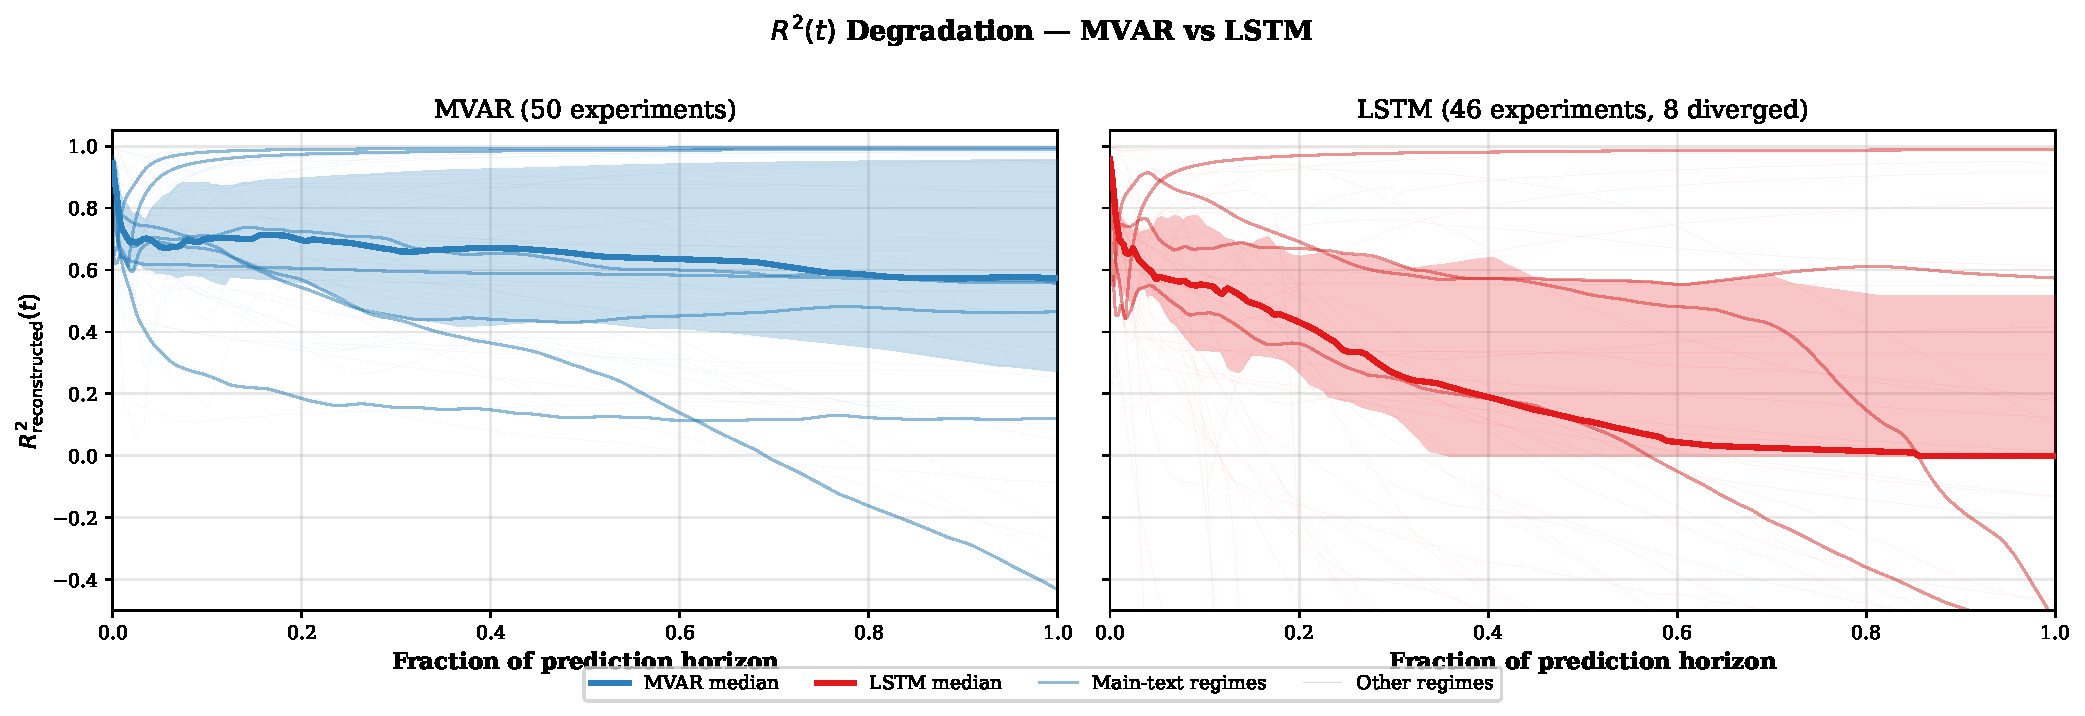
\includegraphics[width=0.95\textwidth]{../Thesis_Figures/appF_r2_degradation_combined.pdf}
\caption{$R^2(t)$ degradation for all systematic experiments.
Left (blue): MVAR\@.  Right (red): LSTM\@.
Faint = individual runs, bold = median, shading = IQR\@.
The aggregate curves exclude diverged LSTM experiments
(final $R^2<{-}2$), whose individual traces remain visible but are
clipped at the axis boundary.}
\label{fig:appF_r2_degradation_combined}
\end{figure}

% -----------------------------------------------------------------------
\section{WSINDy identification for extended regimes}
\label{sec:regime_wsindy_extended}
% -----------------------------------------------------------------------

WSINDy identification was performed only on the nine primary benchmark
regimes (Chapter~\ref{ch:wsindy_results}); extending the identification
pipeline to the remaining configurations is left for future work
(Section~\ref{sec:future_work}).  The EF-ROM forecast $R^2$ values for
all regimes are recorded in Table~\ref{tab:full_regime_catalogue} above.
